\documentclass[a4paper, 15pt]{article}
\usepackage[utf8]{inputenc}
\usepackage{hyperref}
\usepackage{nth}
\usepackage{graphicx}
\usepackage{amsmath}
\usepackage{amssymb}
\usepackage{commath}
\usepackage{algorithm}
\usepackage{algpseudocode}
\usepackage{subcaption}
\usepackage{cite}
\DeclareMathOperator*{\argmax}{argmax} 
\usepackage[square, numbers, comma, sort&compress]{natbib}
\date{\vspace{-5ex}}

\begin{document}
	\graphicspath{{images/}}
	\thispagestyle{empty}
	\begin{center}
		{\fontsize{30}{50}\selectfont CLOUD REMOVAL IN \linebreak \linebreak HYPERSPECTRAL IMAGES}
	\end{center}
	\begin{center}
	\end{center}
	\begin{center}
		{\fontsize{20}{20}\selectfont B.Tech Thesis Project \linebreak by \linebreak ANIRBAN MITRA \linebreak \linebreak 14EE10004}
	\end{center}
	\begin{center}
	\end{center}
	\begin{center}
		{\fontsize{20}{20}\selectfont Under the supervision of \linebreak \textbf{Dr. Rajiv Ranjan Sahay} \linebreak (Department of Electrical Engineering, IIT Kharagpur)}
	\end{center}
	%Inserting Image
	\begin{figure}[h]
		\centering
		
\includegraphics[scale=1.2]{kgplogo.png}
		\label{fig:kgplogo}
	\end{figure}
	\begin{center}
		{\fontsize{20}{20}\selectfont Department of Electrical Engineering \linebreak Indian Institute of Technology Kharagpur \linebreak 
			Kharagpur - 721302, India}
	\end{center}
	\newpage
	\setcounter{page}{1}
	\begin{center}
		{\fontsize{40}{50}\selectfont Abstract}
	\end{center}
	\par 
	Cloud Coverage is a major problem in the optical remote sensing imagery. Hence automated cloud detection and cloud removal is an important step needed in remote sensing image processing. After detection of the cloud mask, successful reconstruction of the occluded region is a major challenge. For successful in-painting, there exists various algorithms which are based on texture synthesis, PDE based in-painting, Hybrid in-painting etc. The algorithm explored to in-paint the image is based on Sparse Representation Modelling\cite{1}. There has been a growing use in the sparse representation of signals in fields of in-painting, feature extraction, de-noising etc as described in \cite{2}. By using an over-complete dictionary that contain prototype signal atoms, the objective signals can be described as the linear sparse combination of these target atoms. For inpainting gradient descent algorithm is used using Gaussian Markov Random Field as a prior. This prior would help in diffusion based inpainting of the image. Further I have explored Total Variation(TV) inpainting which uses the Split Bregman method to inpaint images as described in \cite{5}.
	\par
%	\newpage
%	\begin{center}
%		{\fontsize{40}{50}\selectfont Representation of Sparse Signals}
%	\end{center}
%	\par 
%	Sparse dictionary learning is a learning method aiming to find of a sparse representation of the target signal in the form of a linear combination of atoms of the dictionary. These atoms form the required dictionary. This sparse representation allows the dimensionality of the signals being represented to be higher than that of the signals being observed.
%	\par
%	\par
%	On using an over-complete dictionary that contains signal-atoms, signals are best described by sparse linear combinations of these signal-atoms. Sparse representation have many uses that include compression, feature extraction, etc. Designing dictionaries to fit the model can be done initially by either selecting either from one of the transforms of the original signal and then suitably updating it the fit the original signal. 
%	\par
%	\par
%	K-SVD algorithm is explored, that alternates between updating the dictionary and the sparse coded vector. The update of the dictionary columns is par with an update of the sparse coded vector speeds up the convergence of the objective function. The metric used in \cite{2} as a measure of the stopping criteria is the Mean Squared Error (MSE). K-SVD algorithm provided good results for image de-noising but failed for large scale image in-painting, as the number of unknown pixels’ increases.
%	\par
%	\begin{figure}[h]
%		\centering
%		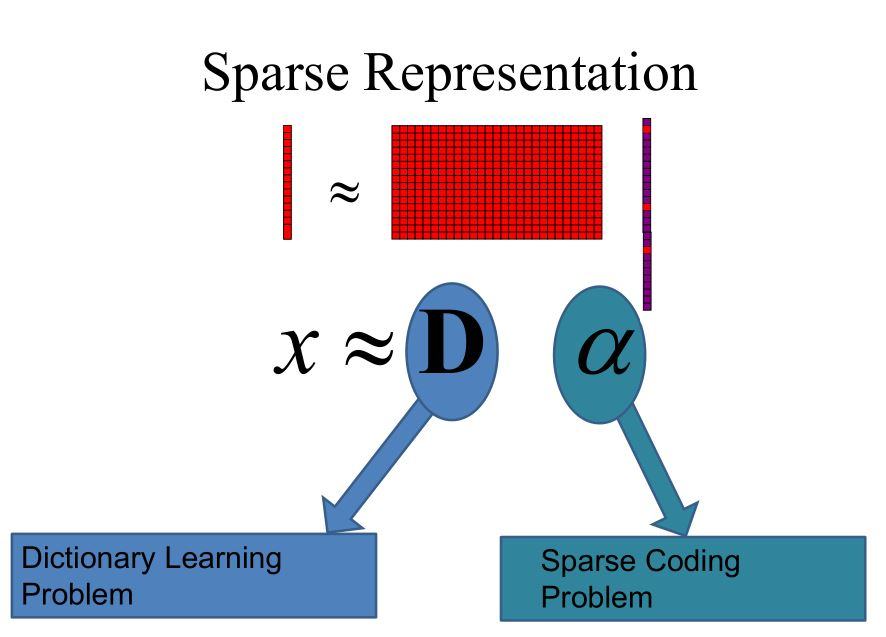
\includegraphics[scale=0.5]{sparse.png}
%		\caption{Sparse Representation}
%		\label{fig:sparse}
%	\end{figure}
%	\newpage
%	\begin{center}
%		{\fontsize{20}{30}\selectfont The Steps Involved are:}\
%	\end{center}
%	\begin{enumerate}
%		\item Detection Of Clouds to form a Mask
%		\item Inpainting of the Occluded Portions in the Original Image
%	\end{enumerate}
	\newpage
	\begin{center}
		{\fontsize{20}{30}\selectfont Detection Of Clouds}\
	\end{center}
	\par
	For Cloud Detection, I used super-pixel segmentation which divides the image into $N$ cluster based on similarity of pixels. It uses simple linear iterative clustering algorithm to group pixels into regions with similar values. The mask generated is passed to the active contour algorithm which segments the image in a mask which contains cloudy and non-cloudy regions.
	\par
	\begin{figure*}[!h]
		\centering 
		\begin{tabular}{cc}
			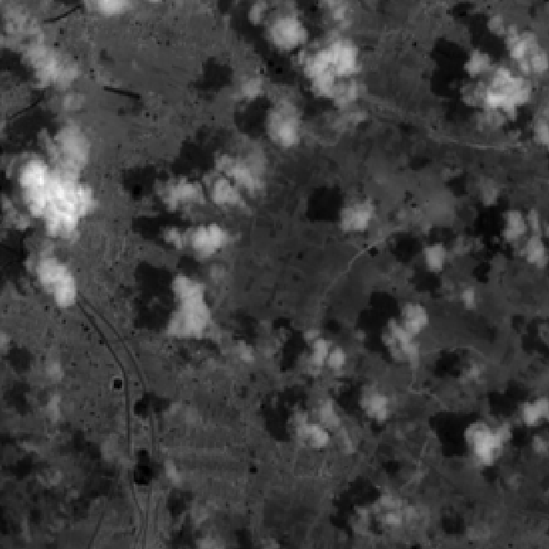
\includegraphics[width=6cm, height=6cm]{cloudSample.png} &\hspace{-8pt}
			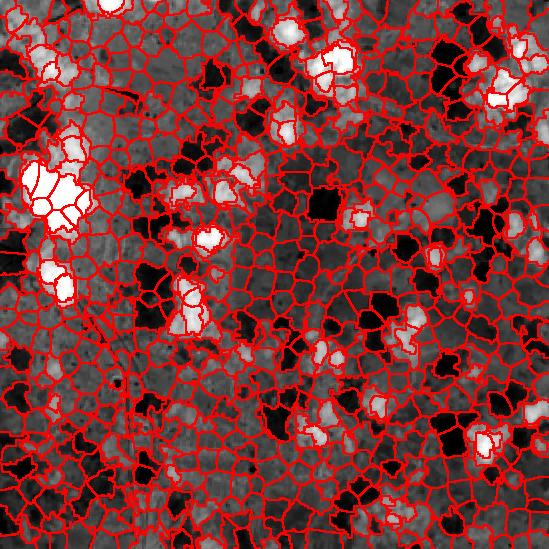
\includegraphics[width=6cm, height=6cm]{patches.jpg}\\
			(a) & (b) \\ \\
			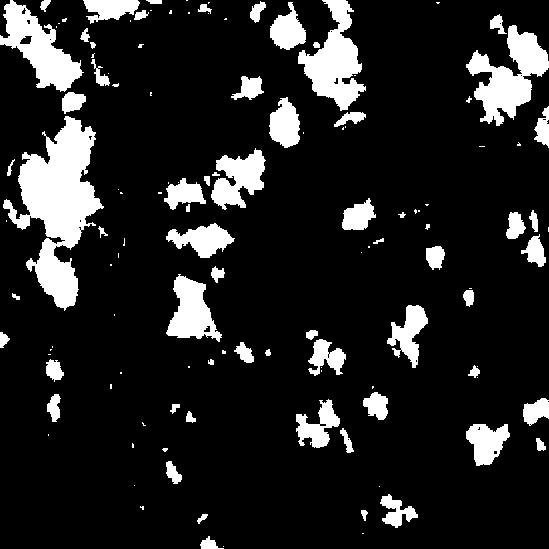
\includegraphics[width=6cm, height=6cm]{cloudMask.jpg} &\hspace{-8pt}
			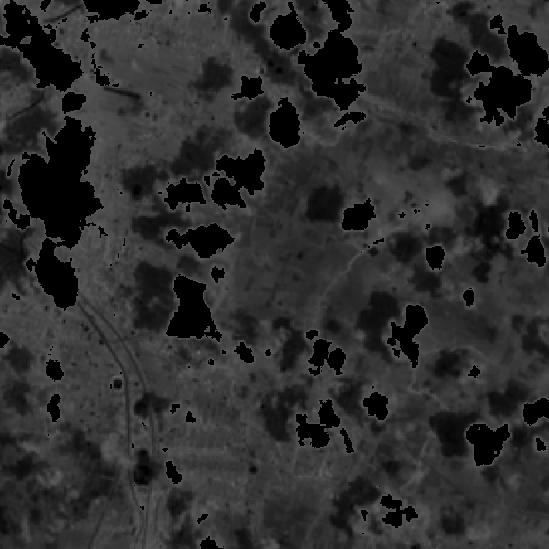
\includegraphics[width=6cm, height=6cm]{final.jpg}\\
			(c) & (d)
		\end{tabular}
		\caption{(a) Original Cloud Image, (b) Super Pixel Image, (c) Mask Formed, (d) Occluded Portion in Original Image.}
	\end{figure*}
	\newpage
	\begin{center}
		{\fontsize{20}{30}\selectfont Reconstruction Of the Occluded Portions}\
	\end{center}
	\par
	For reconstruction Sparse Representation Modelling is used. Sparse Representation theory says that sparse signals can be exactly reconstructed from small number of elementary atoms. Sparse Dictionary Learning is a representation learning which aims at finding a sparse representation of the input data in the form of a linear combination of basic elements. These elements are called atoms and they compose a dictionary. Given a set of training examples we aim to find the dictionary that leads to best representation of each member under strict sparsity constraints. Thus given an overcomplete dictionary, a target signal y can be represented as a sparse linear combination of dictionary atoms 
	\par
	\begin{equation}
	Y = DX
	\end{equation}
	\par 
	where X is a sparse coded vector, Y the set of original signals and D, the overcomplete dictionary. Figure.5 shows the relation between Y, D and X.
	\par
	\par 
	For finding the sparse coded vector using OMP under the constraints,
	\begin{equation}
	\min_{x}\norm { Y - DX}^2_{2}  \quad subject \quad to \quad \norm {x}_{0} \leq T
	\end{equation}
	where $||.||_{0}$ represents the $L-0$ norm(Quasi norm) or the number of non-zero values in the signal. Here It is maximum sparsity taken. A similar objective can alternately be met by considering the MSE being less than some threshold value.
	\begin{equation}
	\min_{D, X}\sum_{i}\norm { x }_{0} \quad subject \quad to \quad \norm { Y - DX}^2_{2} \leq \epsilon
	\end{equation}
	\par
	\par 
	We use algorithms which greedily approximates solutions like Matching Pursuit and Orthogonal Matching Pursuit to find the approximate sparse coded vector X. The basis pursuit algorithm is also a representative algorithm similar to OMP that solves the problem by replacing the L0 -norm with an $L1$ norm.
	\par
	\newpage
	\begin{center}
		{\fontsize{20}{30}\selectfont Orthogonal Matching Pursuit Algorithm for Finding Sparse Coded Vector}\
	\end{center}
	\par
	Orthogonal Matching Pursuit (OMP) is a representation algorithm for finding the sparse coded vector. It involves finding the best matching projection of multidimensional data onto the span of a dictionary. As it is a greedy algorithm, on every step it selects the atom with the highest correlation with the existing method. On selecting the atom, the signal is projected orthogonally to the selected atoms and the residual is re-calculated. This method is repeated until stopping criterion is met. The steps given below describes the algorithm. 
	\par

	\begin{algorithm}
		\caption{ORTHOGONAL MATCHING PURSUIT}
		\begin{algorithmic}[1]
			\State Input: Dictionary $D$, signal $\underline{x}$, target sparsity $K$ or target error $\epsilon$	
			\State Output: Sparse Representation $\underline{\gamma}$ such that $\underline{x}$ $\approx$ $D\underline{\gamma}$
			\State Init: Set $I := ()$, $\underline{r} := \underline{x}$, $\underline{\gamma} := \underline{0}$
			\While {stopping criterion not met}
				\State	$\hat{k} := \argmax_{k}{\abs{\underline{d^{T}_{k}} \underline{r}}} $
				\State $I := (I, \hat{k})$
				\State $\underline{\gamma_{I}} := (D_{I})^{+}\underline{x} $
				\State $\underline{r} := \underline{x} - D_{I}\underline{\gamma_{I}} $
			\EndWhile
		\end{algorithmic}
	\end{algorithm}
	\newpage
	\begin{center}
		{\fontsize{20}{30}\selectfont KSVD Algorithm}\
	\end{center}
	\par
	For finding the optimal Dictionary, K-SVD algorithm is used. K-SVD, a dictionary learning algorithm is used for creating the optimal dictionary for sparse representations, via the singular value decomposition approach \cite{1}. SVD decomposition is used to maximize the similarity of the existing dictionary. K-SVD is similar to the k-means clustering method as it works by iteratively alternating between sparse coding the target signal on basis of the current dictionary, and simultaneously updating the atoms to fit the signal properly.
	\par
	\begin{figure}[h]
		\centering
		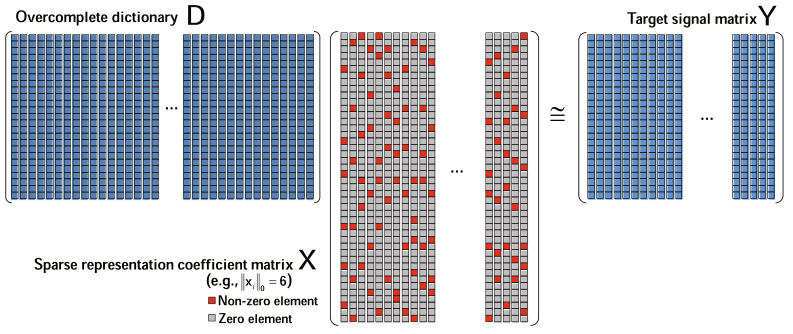
\includegraphics[scale=0.6]{svd.png}
		\caption{Sparse Signal Representation of Y}
		\label{fig:svd}
	\end{figure}
	\par
	The update of atoms in the dictionary is combined with the simultaneous update of the sparse coded vector to make convergence faster. The K-SVD algorithm is flexible in the sense that it can work with almost any matching pursuit algorithms. 
	\par
	\begin{figure}[h]
		\centering
		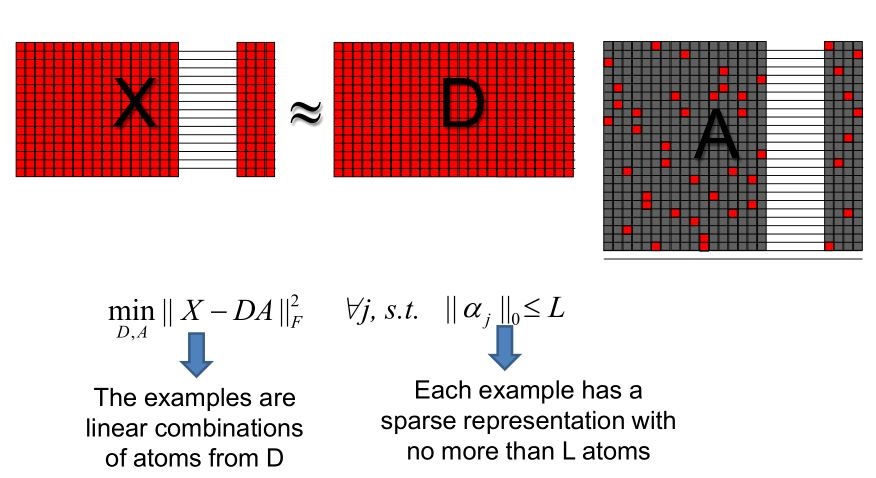
\includegraphics[scale=0.5]{KSVD.JPG}
		\caption{Objective Function For KSVD}
		\label{fig:KSVD}
	\end{figure}
	\newpage
	\par
	The dictionary updated in an iterative manner as depicted in the flowchart: 
	\par 
	\begin{figure}[h]
		\centering
		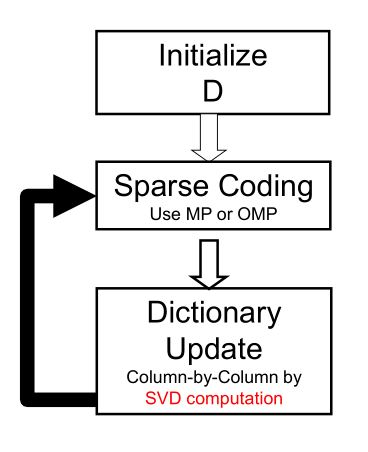
\includegraphics[width=0.35 \textheight]{flowchartksvd.JPG}
		\caption{Objective Function For KSVD}
		\label{fig:flowchartksvd}
	\end{figure}
	\newpage
	\begin{center}
		{\fontsize{20}{30}\selectfont Results in Denoising of Images}\
	\end{center}
	\par
	This KSVD algorithm was applied for the de-noising of images. The results obtained were in par with other de-noising algorithms. The noise added was Gaussian noise. 
	\par
	\par
	This same process was repeated for a RGB image by taking the concatenation of different bands as the vector but the results obtained were not that good. 
	\par
	\par
	This method was repeated taking a patch size of $8*8$ throughout the image. On taking distinct patches the overall results were not up to the mark, so overlapping patches were taken to train the Dictionary well. 
	\par
	\begin{figure}[!h]
		\centering 
		\begin{tabular}{cc}
			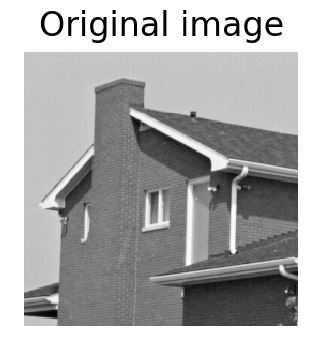
\includegraphics[width=6cm, height=6cm]{Original_KSVD.JPG} &\hspace{-8pt}
			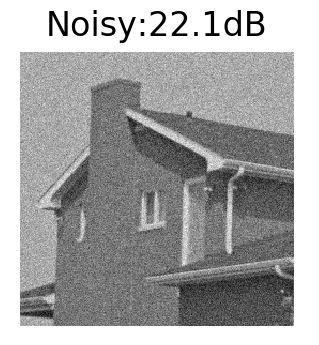
\includegraphics[width=6cm, height=6cm]{Noisy_22_1dB_KSVD.JPG}\\
			(a) & (b) \\
		\end{tabular}
		\begin{tabular}{c}
			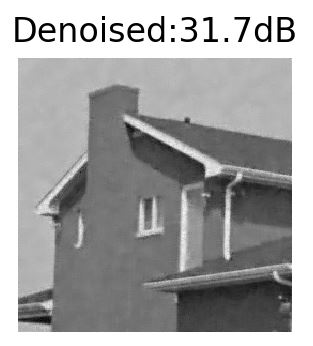
\includegraphics[width=6cm, height=6cm]{Denoised_31_7_KSVD.JPG}\\ 
			(c)
		\end{tabular}
		\caption{(a) Original Image, (b) Noisy Image with Gaussian Noise added, (c) Denoised Image.}
	\end{figure}
	\par
	Thus we see that MSE denoising is not up to the mark. 
	\par
	\newpage
	\begin{center}
		{\fontsize{20}{30}\selectfont Changing the Metric to SSIM}\
	\end{center}
	\par
	The original metric used in KSVD algorithm was the Mean Squared Error (MSE), as it is a popular metric used in most image processing algorithms. However, it is not that accurate as MSE cannot provide high visual quality in images. Thus it may not be appropriate to use MSE as quality measure in in-painting. 
	\par
	\par
	Another well-known metric measure is the Structural Similarity Index (SSIM), which is used for quality measure in Image Processing. The definition of the SSIM index is first extended to measure the similarity between signals via their statistical equivalents. The SSIM between two signals x and y depends on the sample means, sample variance and the cross-variance between x and y. 
	\par
	\par
	Thus the SSIM between the two signals is given by the equation: 
	\par
	\begin{equation}
	SSIM(x, y) = \left( \frac{2\mu_{x}\mu_{y} + C_{1}}{\mu^2_{x}+\mu^2_{y} + C_{1}} \right)\left( \frac{2\sigma_{xy} + C_{2}}{\sigma^2_{x} + \sigma^2_{y} + C_{2}}\right)
	\end{equation}
	\par
	Thus instead of using MSE as a criterion in OMP for obtaining the sparse coded vector SSIM is used as a metric. Thus the objective function gets converted to  
	\par
	\begin{equation}
	\max_{x_{i}} SSIM(y_{i}, Dx_{i}) \quad subject \quad to \quad \norm {x}_{0} \leq T
	\end{equation}
	\par
	That is, we have to find a sparse coded vector such that the SSIM is maximum and also the sparsity does not exceed T. Thus SSIM metric will be the stopping criteria for the OMP algorithm. Thus on modifying the KSVD algorithm again using SSIM as a metric we apply it on de-noising of images \cite{3}. 
	\par
	\newpage
	\begin{figure}[!h]
		\centering 
		\begin{tabular}{cc}
			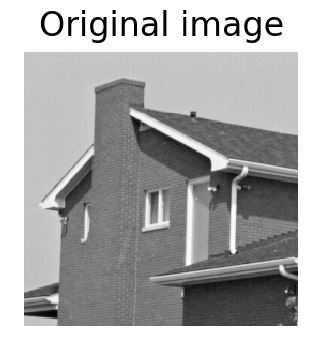
\includegraphics[width=6cm, height=6cm]{Original_KSVD.JPG} &\hspace{-8pt}
			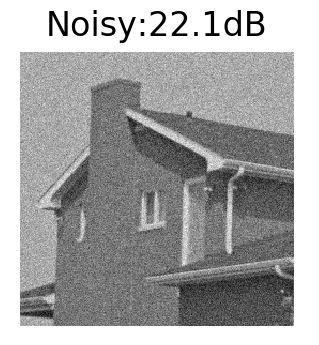
\includegraphics[width=6cm, height=6cm]{Noisy_22_1dB_KSVD.JPG}\\
			(a) & (b) \\
		\end{tabular}
		\begin{tabular}{c}
			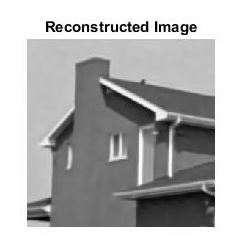
\includegraphics[width=6cm, height=6cm]{SSIM_rec.JPG}\\ 
			(c)
		\end{tabular}
		\caption{(a) Original Image, (b) Noisy Image with Gaussian Noise added, (c) Denoised Image by SSIM 33.7dB.}
	\end{figure}
	\newpage
	\begin{center}
		{\fontsize{20}{30}\selectfont SSIM Calculation}\
	\end{center}
	\par
	The SSIM metric is generally calculated in 2 different ways 
	\par
	\begin{itemize}
		\item Using the dependance of means and standard deviation on pixel $p$
		\item By ommiting the dependence on pixel p and calculating the mean and standard deviation with a Gaussian filter with standard deviation $\sigma_{G}$
	\end{itemize}
	The expression of $SSIM$ can be written as:
	\begin{equation}
	SSIM(x, y) = \left( \frac{2\mu_{x}\mu_{y} + C_{1}}{\mu^2_{x}+\mu^2_{y} + C_{1}} \right)\left( \frac{2\sigma_{xy} + C_{2}}{\sigma^2_{x} + \sigma^2_{y} + C_{2}}\right)  = l(p).cs(p)
	\end{equation}
	\par
	For calculations via Gaussian Filter, given a patch $P_{x}$ 
	\par
	\begin{equation}
	\mu_{x}(p) = G_{\sigma_{G}}\circledast P_{x}
	\end{equation}
	\begin{equation}
	\sigma^2_{x}(p) = G_{\sigma_{G}}\circledast P^2_{x} - \mu^2_{x}(p)
	\end{equation}
	\begin{equation}
	\sigma_{xy}(p) = G_{\sigma_{G}}\circledast (P_{x}.P_{y})- \mu_{x}(p)\mu_{y}(p)
	\end{equation}
	where, $P_{x}$ is a patch centered at pixel p, '$\circledast$' denotes a convolution, '.' a point-wise multiplication. The values of $\mu_{x}(p)$ and $\sigma^2_{y}(p)$ can be computes similarly. The dimension of the filter is taken by the $6\sigma+1$ principle so that it has a coverage over $95\% $.
	\newpage
	\begin{center}
		{\fontsize{20}{30}\selectfont Using Gradient Descent for De-Bluring}\
	\end{center}
	\par
	As the performance of SSIM does not come up to the mark, I checked whether it performs basic operations like deblurring in images, Thererfore a comparison was made between the performance of SSIM and MSE to see which one performs better. \par
	Thus a comparison was based on 3 methods:
	\begin{enumerate}
		\item Gradient Descent using Mean Squared Loss as Objective Function.
		\item Gradient Descent using SSIM with Gaussian Filter as Objective Function.
		\item Gradient Descent using SSIM without Gaussian Filter as Objective Function.
	\end{enumerate}
	\par The update equation in Gradient Descent is as:
	\begin{equation}
	\theta^{k+1} = \theta^{k} - \eta \circledast \nabla_{\theta}J(\theta)
	\end{equation}
	where $J(\theta)$ is the objective function and $\eta$ is the learning rate parameter that determines the size of steps we take to reach the minimum. 
	\par
	\par
	As we see from the below images that the weighted sum of MSE and SSIM performs the best in the above examples. This is because int MSE, the rate of convergence is really fast while on the other hand SSIM converges very slowly. SSIM is needed to reconstruct the structural components of the images. The graphs below show the performance of the three Objective Functions. 
	\par
	\newpage
	\graphicspath{{results/}}
	\begin{figure}[!h]
		\centering
		\begin{tabular}{cc}
			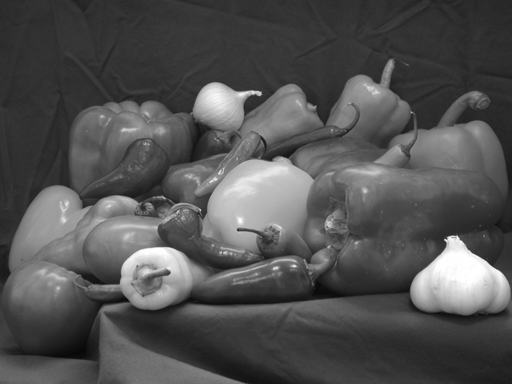
\includegraphics[width=7cm, height=5.3cm]{pepper.jpg} &\hspace{-8pt}
			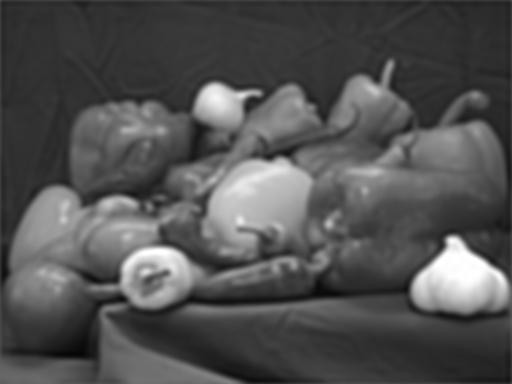
\includegraphics[width=7cm, height=5.3cm]{Original_Blured.jpg}\\
			(a) & (b) \\ 
			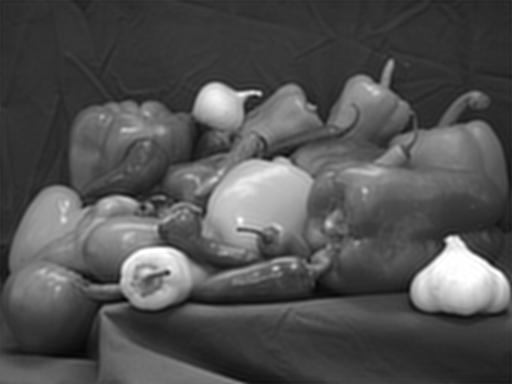
\includegraphics[width=7cm, height=5.3cm]{MSE_reconstruction.jpg} &\hspace{-8pt}
			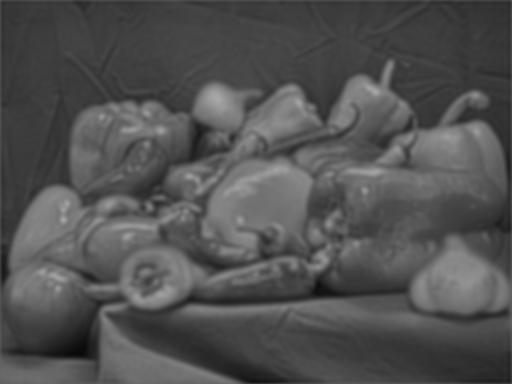
\includegraphics[width=7cm, height=5.3cm]{SSIM_Reconstruction_Gaussian.jpg}\\
			(c) & (d) \\ 
			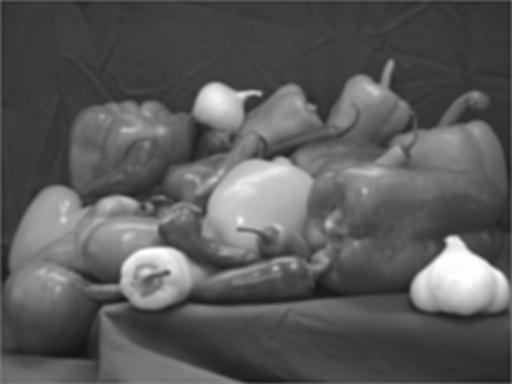
\includegraphics[width=7cm, height=5.3cm]{SSIM_Reconstruction_Simple.jpg} &\hspace{-8pt}
			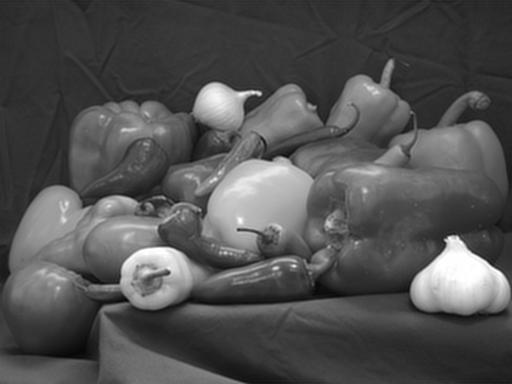
\includegraphics[width=7cm, height=5.3cm]{ssimL2Rec.jpg}\\
			(e) & (f) \\
		\end{tabular}
		\caption{(a) Original Image Ground Truth, (b) Blurred Image, (c) Image Reconstructed via MSE, (d) Image Reconstructed via SSIM using Gaussian Filter, (e) Image Reconstructed via SSIM without using Gaussian Filter, (f) Image Reconstructed via weighted sum of MSE and SSIM.}
	\end{figure}

	\newpage	
	\begin{figure}[h]
		\centering
		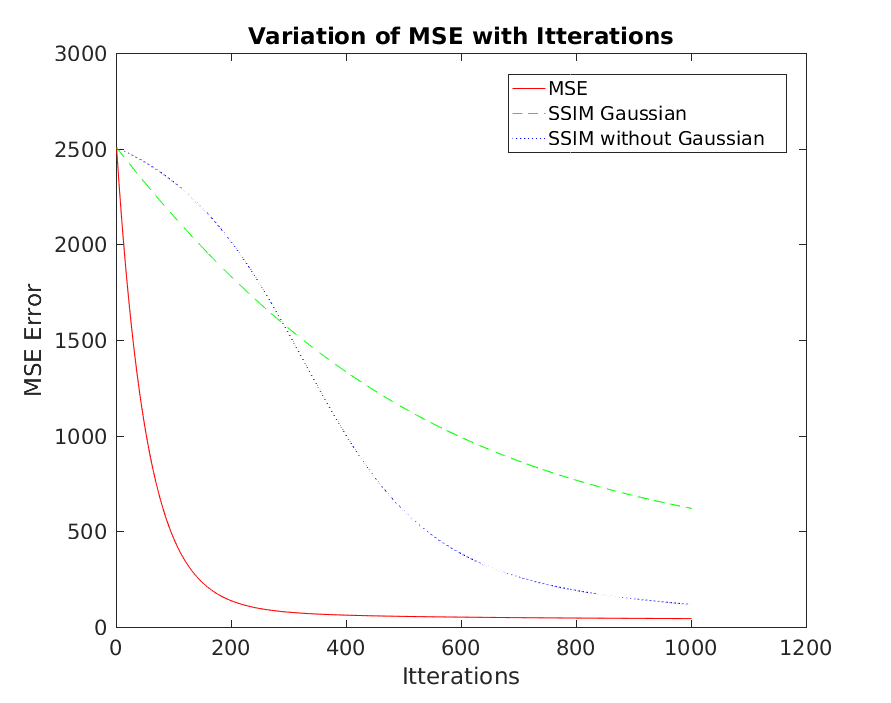
\includegraphics[scale=0.6]{Variation_of_MSE_with_Itterations.png}
		\caption{Variation Of MSE for 3 Objective Functions for 1000 itterations}
		\label{fig:Variation_of_MSE_with_Itterations}
	\end{figure}
	\begin{figure}[h]
		\centering
		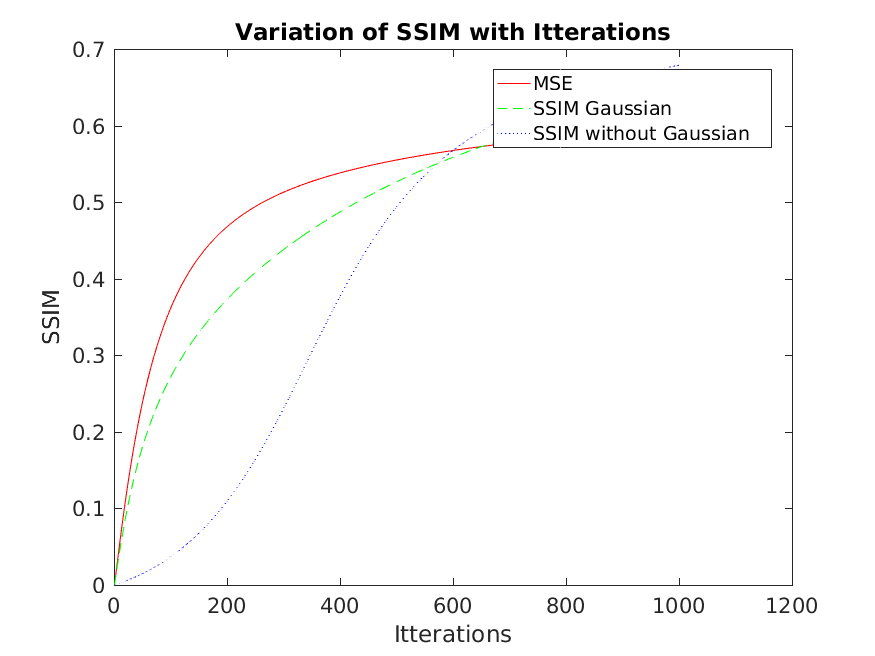
\includegraphics[scale=0.6]{Variation_of_SSIM_with_Itterations.png}
		\caption{Variation Of SSIM for 3 Objective Functions for 1000 itterations}
		\label{fig:Variation_of_SSIM_with_Itterations}
	\end{figure}
	\newpage
	\begin{center}
		{\fontsize{20}{30}\selectfont Using Gradient Descent for Inpainting}\
	\end{center}
	\par
	On applying of gradient descent for inpainting we use the GMRF model for diffusion inpainting.
	Diffusion inpainting makes use of the information in the neighbouring pixels to in-paint an unknown pixel. So the inpainting equation becomes. 
	\par
	\begin{equation}
	Y = O.*X
	\end{equation}
	where $Y$ is our observation, $X$ is our estimation and $O$ is the mask. Thus in gradient descent the update equation becomes,
	\begin{equation}
	\theta^{k+1} = \theta^{k} - \eta\circledast(\nabla_{\theta}J(\theta) + lambda*prior)
	\end{equation}
	\par
	The GMRF model taken is the squared difference of the neighboiring pixels, 
	\par
	\begin{equation}
	\begin{split}
	GMRF(i, j) = (X(i,j) - X(i-1, j))^2 + (X(i,j) - X(i+1, j))^2 + \\ (X(i,j) - X(i, j-1))^2 + (X(i,j) - X(i, j+1))^2
	\end{split}	
	\end{equation}
	The derivative of the GMRF is calculated as:
	\begin{equation}
	\begin{split}
	\nabla GMRF(i, j) = 2*((X(i,j) - X(i-1, j)) + (X(i,j) - X(i+1, j)) + \\ (X(i,j) - X(i, j-1)) + (X(i,j) - X(i, j+1)))
	\end{split}
	\end{equation}
	\newpage
	\begin{center}
		{\fontsize{20}{30}\selectfont Results Obtained}\
	\end{center}
	\begin{figure}[!h]
		\centering 
		\begin{tabular}{cc}
			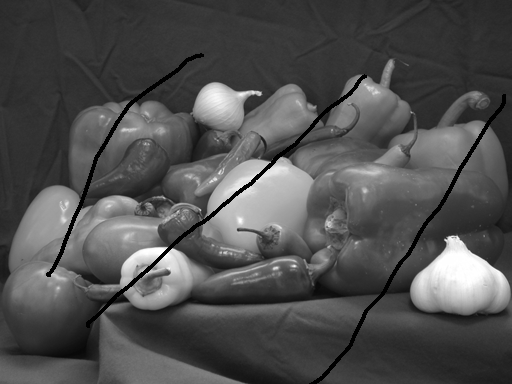
\includegraphics[width=7cm, height=5.3cm]{observationGMRF.png} &\hspace{-8pt}
			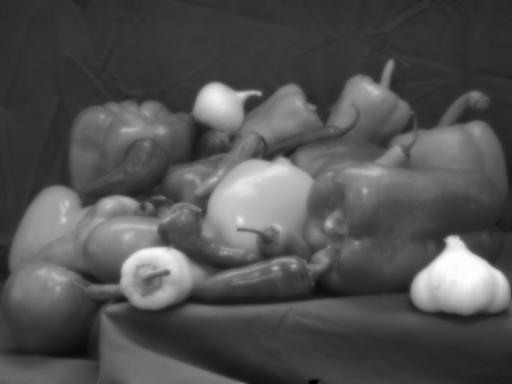
\includegraphics[width=7cm, height=5.3cm]{ssimSimpleRec.png}\\
			(a) & (b) \\
		\end{tabular}
		\begin{tabular}{c}
			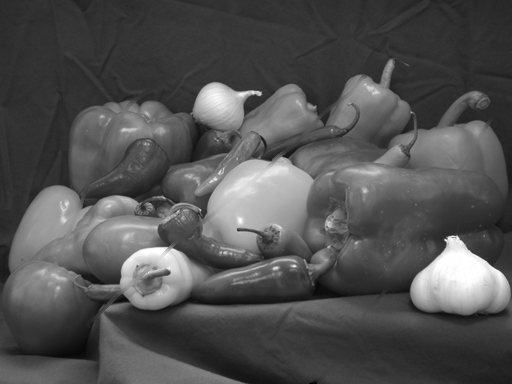
\includegraphics[width=7cm, height=5.3cm]{bestOutGMRF.png}\\ 
			(c)
		\end{tabular}
		\caption{(a) Observation Image which has to be In-Painted, (b) Estimated Image after Inpainting, (c) Output Image.}
	\end{figure}
	\newpage
	\begin{center}
		{\fontsize{20}{30}\selectfont Results on Hyperspectral Images}\
	\end{center}
	\begin{figure}[!h]
		\centering
		\begin{tabular}{cc}
			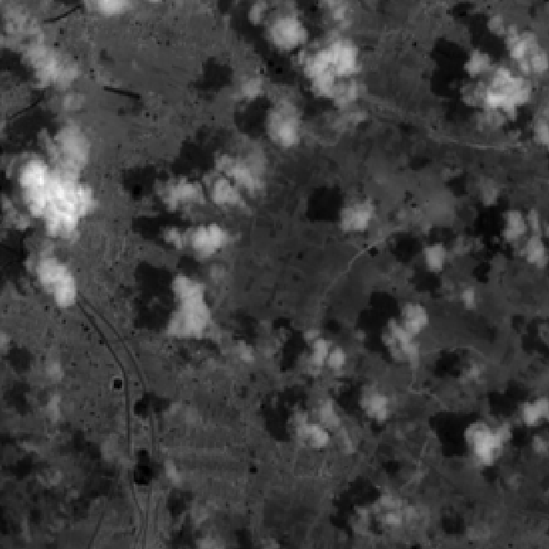
\includegraphics[width=6cm, height=6cm]{cloudSample.png} &\hspace{-8pt}
			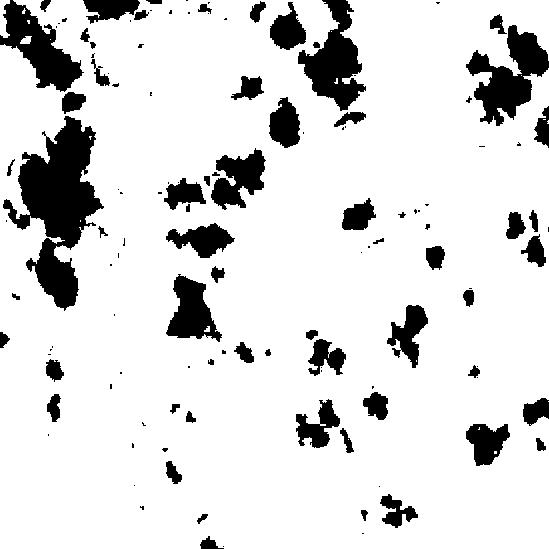
\includegraphics[width=6cm, height=6cm]{cloudMask2.jpg}\\
			(a) & (b) \\ 
			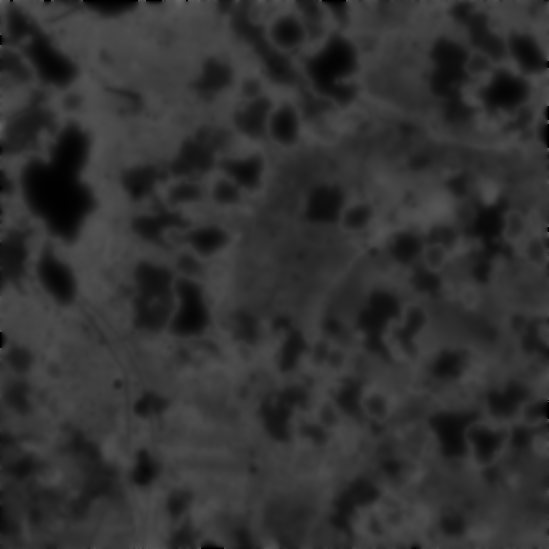
\includegraphics[width=6cm, height=6cm]{CloudInpainted_OrigGMRF.png} &\hspace{-8pt}
			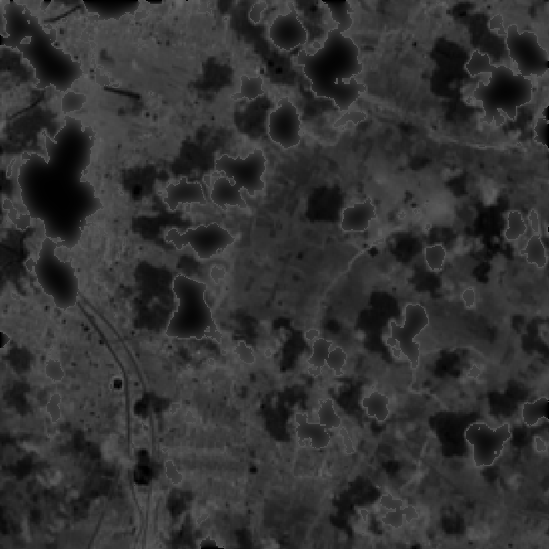
\includegraphics[width=6cm, height=6cm]{CloudInpaintedGMRF.png}\\
			(c) & (d)
		\end{tabular}
		\caption{(a) Cloud sample Image, (b) Cloud Mask, (c) Estimated Image, (d) Best Estimated Image.}
	\end{figure}
	\newpage
	\begin{center}
		{\fontsize{20}{30}\selectfont In-Painting Using Split Bregman Itteration}\
	\end{center}
	\par
	Until now I have used GMRF as the prior, but research shows that TV(Total Variation) as a prior performs well. TV denoising is considered to be one of the best denoising models, but also one of the hardest to compute. However Bregman itteration technique can be used to solve this problem extremley simply and efficiently. Total Variation can be defined as 
	\par
	\par 
	For an image the  TV can be of two types:
	\par
	\begin{itemize}
		\item Isotropic Total Variation
		\begin{equation}
		V(y) = \sum_{i,j}\sqrt{\abs{y_{i+1,j}-y_{i,j}}^2 +\abs{y_{i,j+1}-y_{i,j}}^2}
		\end{equation}
		which for image can be calculated as:
		\begin{equation}
		\min_{u}\sum_{i}\sqrt{(\nabla_{x}u)^2_{i} + (\nabla_{y}u)^2_{i}}
		\end{equation}
		\item Anisotropic Total Variation
		\begin{equation}
		V(y) = \sum_{i,j}\abs{y_{i+1,j}-y_{i,j}} +\abs{y_{i,j+1}-y_{i,j}}
		\end{equation}
		\begin{equation}
		\min_{u}\abs{\nabla_{x}u} + \abs{\nabla_{y}u}
		\end{equation}
	\end{itemize} 
	The Split Bregman Expression can be shown as:
	\begin{equation}
	\min_{d_{x},d_{y},u} \abs{d_{x}} + \abs{d_{y}} + \frac{\mu}{2}\norm{u - O.X}^2_{2} + \frac{\lambda}{2}\norm{d_{x} - \nabla_{x}u - b^{k}_{x}}^2_{2} + \frac{\lambda}{2}\norm{d_{y} - \nabla_{y}u - b^{k}_{y}}^2_{2}
	\end{equation}
	Thus in equation 19 the first $2$ TV terms are solved using a soft thresholding function (shrink operator) while the rest $3$ are solved using gradient descent.
	\begin{algorithm}
		\caption{Split Bregman TV Inpainting}
		\begin{algorithmic}[1]
			\State Initialize $u^{0} = f, and d^{0}_{x} = d^{0}_{y} = b^{0}_{x} = b^{0}_{y} = 0$
		\While {$\norm{u^{k} - u^{k-1}}_2 > tol$}
			\State	$u^{k+1} = Gradient Descent(u^k) $
			\State $d^{k+1}_{x} = shrink(\nabla_{x}u^{k+1} + b^{k}_{x}, 1/\lambda $
			\State $d^{k+1}_{y} = shrink(\nabla_{y}u^{k+1} + b^{k}_{y}, 1/\lambda $
			\State $b^{k+1}_{x} = b^{k}_{x} + (\nabla_{x}u^{k+1} - d^{k+1}_{x})$
			\State $b^{k+1}_{y} = b^{k}_{y} + (\nabla_{y}u^{k+1} - d^{k+1}_{y})$
			\EndWhile
		\end{algorithmic}
	\end{algorithm}
	\newpage
	\begin{center}
		{\fontsize{20}{30}\selectfont Split Bregman Itteration Results}\
	\end{center}
	\begin{figure}[!h]
		\centering 
		\begin{tabular}{cc}
			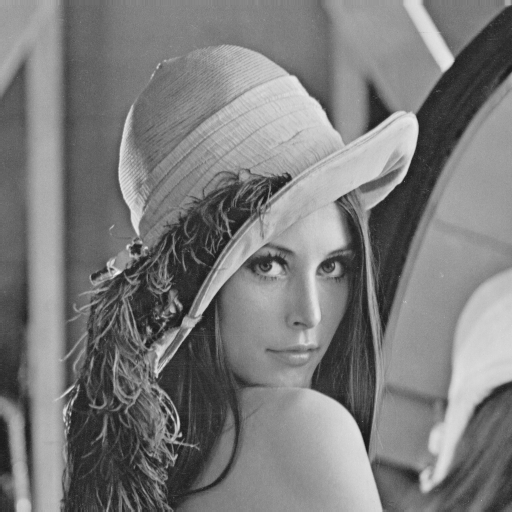
\includegraphics[width=6cm, height=6cm]{Lena512.png} &\hspace{-8pt}
			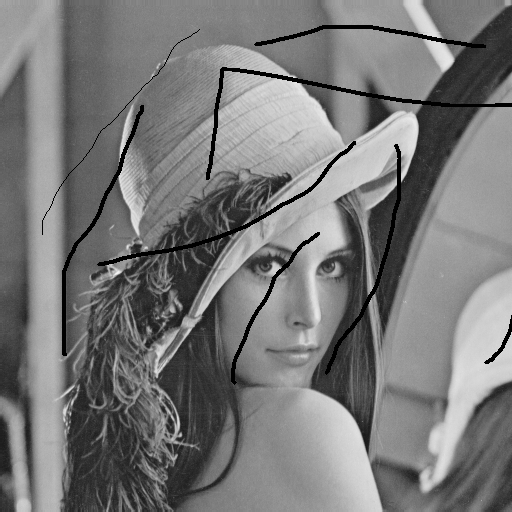
\includegraphics[width=6cm, height=6cm]{observationBregman.png}\\
			(a) & (b) \\
			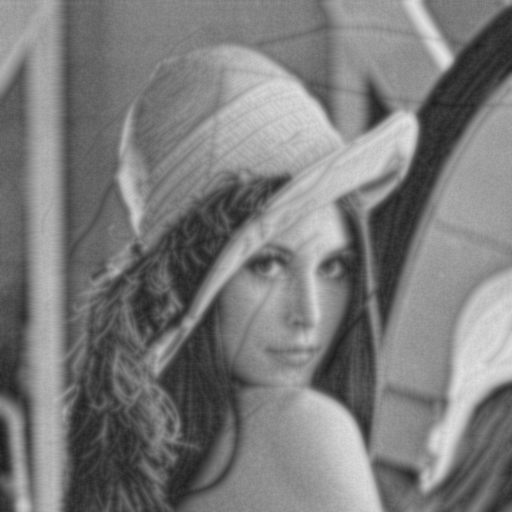
\includegraphics[width=6cm, height=6cm]{estimationBregman.png} &\hspace{-8pt}
			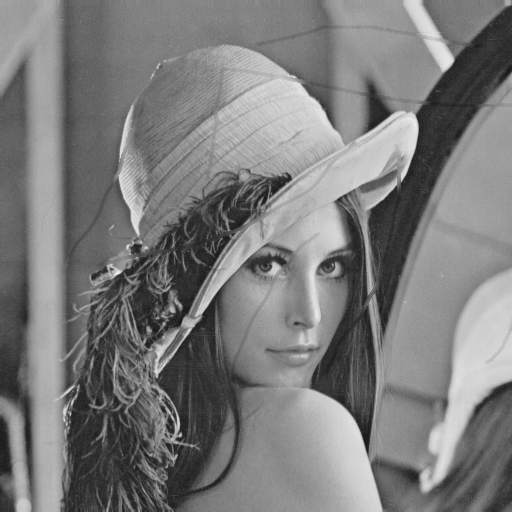
\includegraphics[width=6cm, height=6cm]{bestestimationBregman.png}\\
			(a) & (b) 
		\end{tabular}
		\caption{(a) Observation Image, (b) Image with Scratches which has to be Inpainted, (c) Output Image Generated, (d) Best Output Image keeping features.}
	\end{figure}	
%	\newpage
%	\begin{center}
%		{\fontsize{20}{30}\selectfont Future Work}\
%	\end{center}
%	\par
%	After obtaining the updated dictionary which is trained on the reference patches, the dictionary will be used to predict the target patches that is the patches which needs to be filled. The normal reconstruction from the dictionary gives poor results so patch priority needs to be assigned as discussed in [4]. Thus the missing areas will be filled with certain patches which have higher information contain. This way will ensure that at once each unknown pixel gets in-painted instead of filling up an entire unknown patch at once. As this method is computationally expensive we want to search for faster implementation of the algorithms. 
%	\par
%	\newpage
%	\begin{center}
%		{\fontsize{20}{30}\selectfont Conclusion}\
%	\end{center}
%	\par
%	By comparing the de-noising results obtained by implementing K-SVD with MSE and SSIM we see that the results obtained by using SSIM are better in comparison. MSE does not have high visual quality, while SSIM depends on the statistical parameters. SSIM index can be calculated for some areas as it follows block-wise scheme and not a pixel-wise scheme. To understand the usage of SSIM index for in-painting block-wise procedures are adapted. 
%	\par
	\newpage
	\bibliographystyle{IEEEtran}
	\bibliography{btpRep}
\end{document}